\documentclass[12pt]{report}
\usepackage{fullpage}
\usepackage{pdfpages}

\begin{document}
\title{Sprint 2 Report\\Call Of Adventure}
\author{James Iwamasa(PO)\\Majid Reza Barghi(SM)\\Nickolas Bayt\\Julius Mazer\\Shirley Huang\\Kenneth Bendo}
\date{3-1-17}
\maketitle


\newpage
\section{Actions To Stop Doing}
\begin{itemize}
	\item At this point, we would like to avoid adding any new big features. Most of the main features have been 
implemented, but a lot of them are kind of rough. Rather than add new features, we would like to now polish 
the features we have implemented. 
\end{itemize}

\section{Actions To Start Doing}
\begin{itemize}
	\item Start focusing on style and presentation. 
	\item Make decisive design decisions for the game aspects (how hard battles should be, etc).
	\item Extensive bug testing.
	\item Static asset generation (art).
\end{itemize}

\section{Actions To Keep Doing}
\begin{itemize}
	\item Learning new skills (particularly in css and Unity).
\end{itemize}

\section{Work Completed}
\begin{itemize}
	\item Shop item availability is balanced to user ability.
	\item Quest availability is balanced to user ability.
	\item Partial styling of pages, mostly in terms of format rather than aesthetic. 
	\item User-generated quests.
	\item Item crafting.
	\item Unity game HUD navigation.
	\item Unity game access to database.
	\item Unity game turn system.
	\item Unity game GUARD ability. 
\end{itemize}

\section{Work Not Completed}
\begin{itemize}
	\item Unity game damaging method.
	\item Unity game special attacks. 
	\item Unity game monster AI.
\end{itemize}

\section{Work Completion Rate}
\begin{itemize}
	\item Total Number of User Stories Completed: 8
	\item Total Number of Ideal Work Hours: 59
	\item Total Number of Days in Sprint: 14
	\item Average Work Hours/Day: 4.2
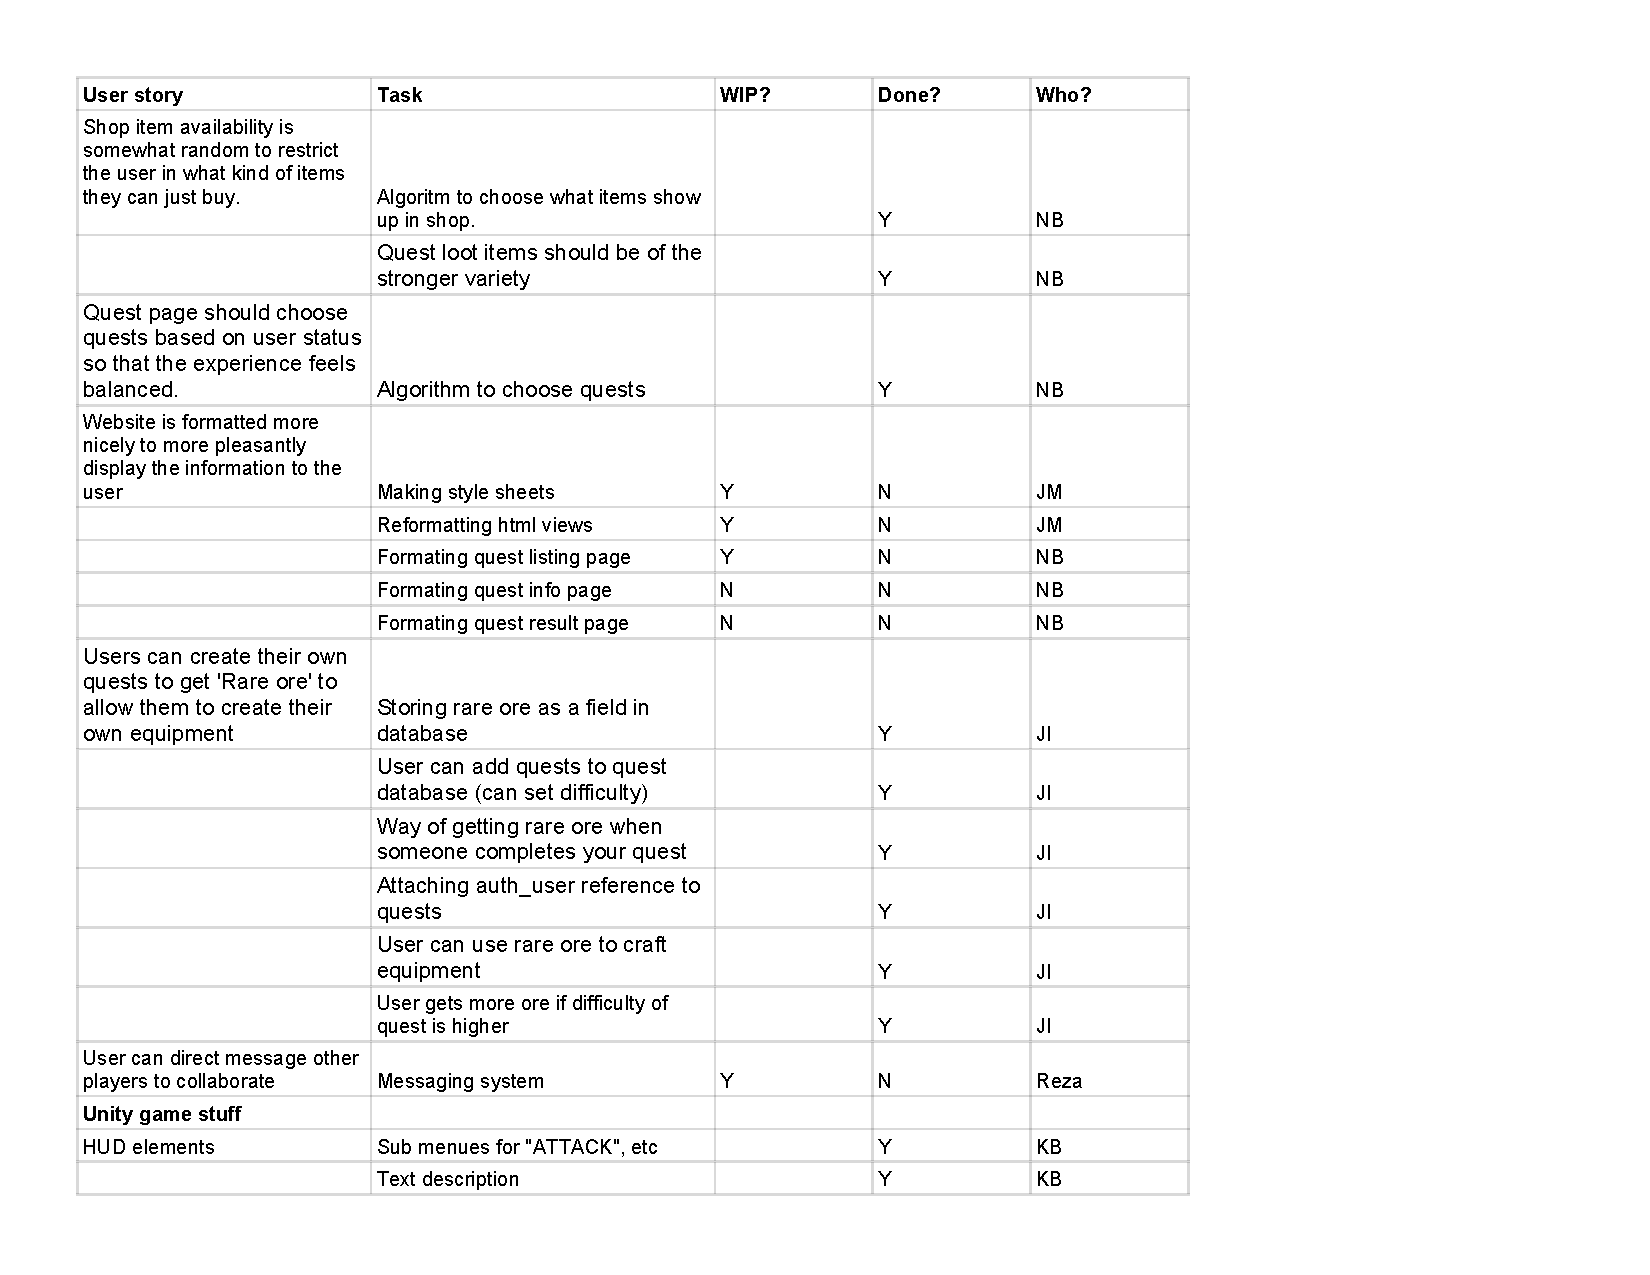
\includepdf[]{sprint2scrumboard.pdf}
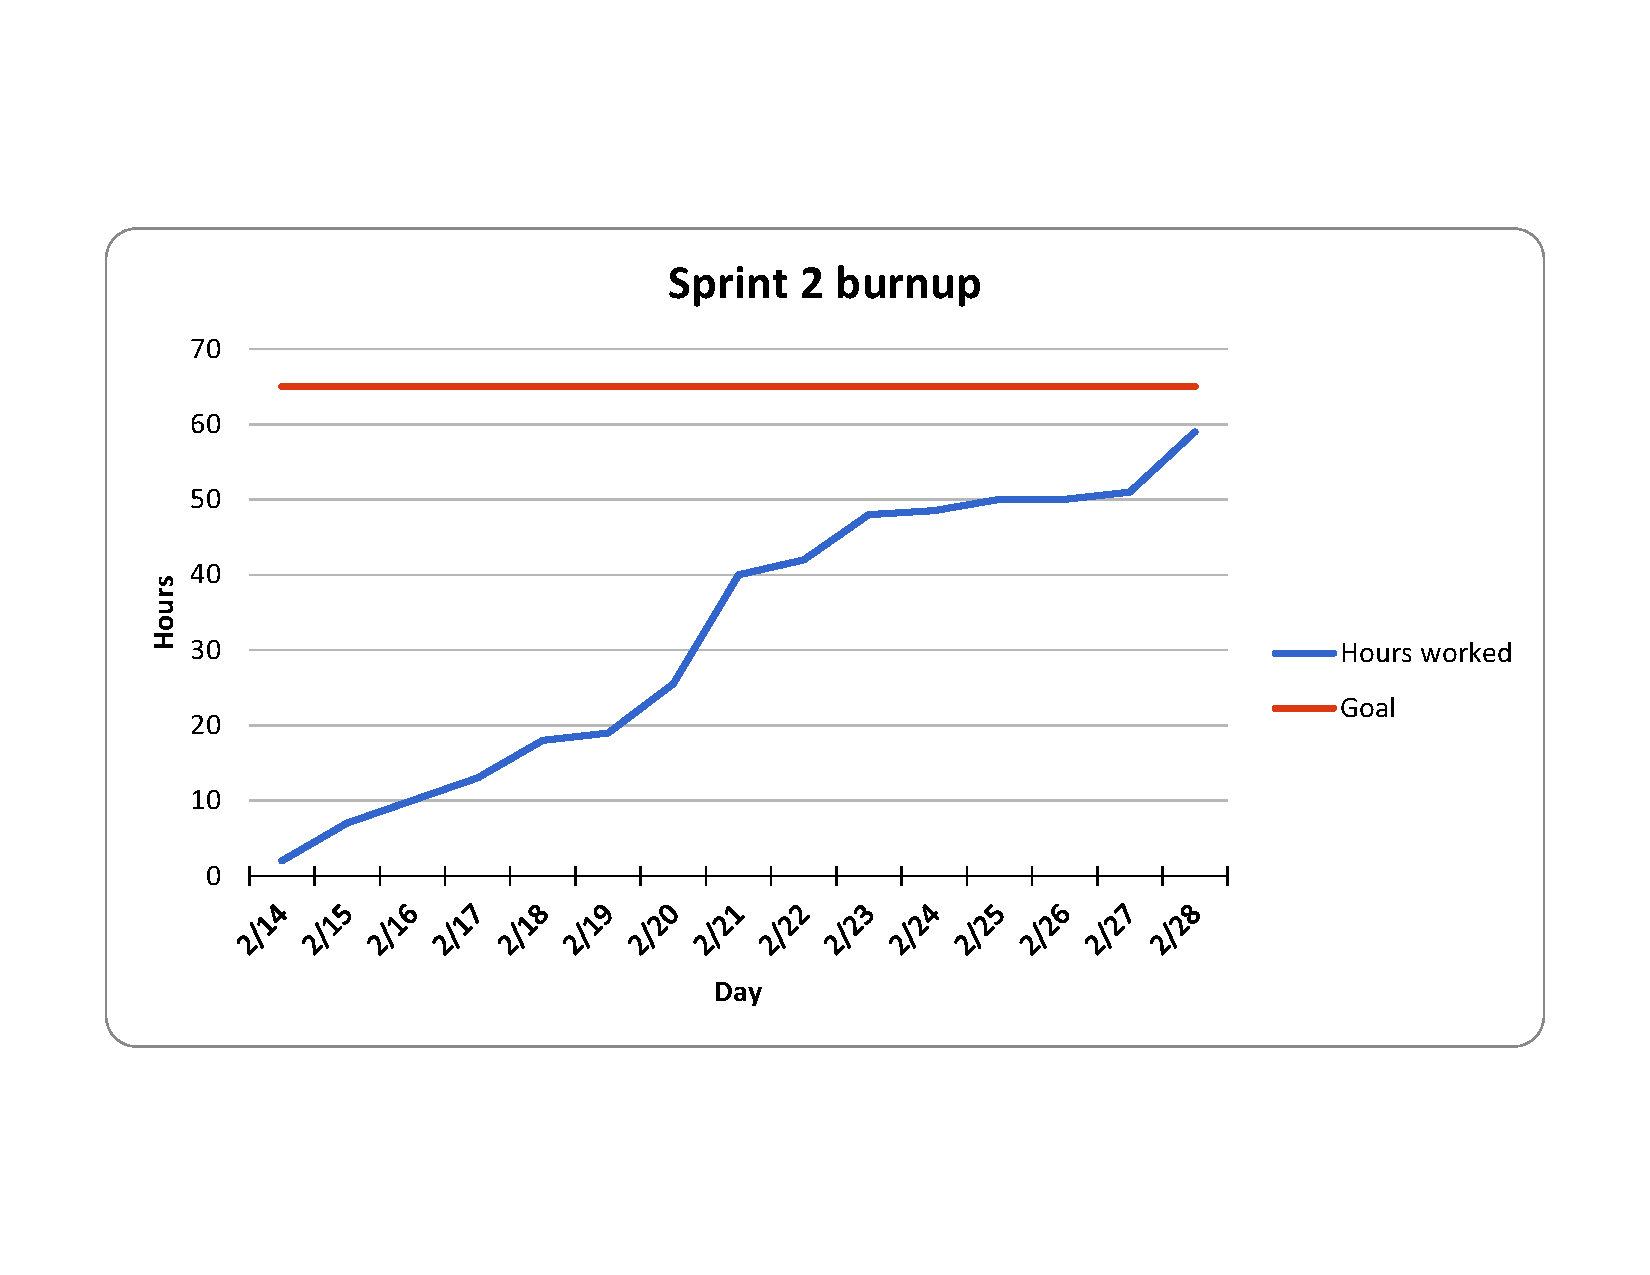
\includepdf[]{sprint2burnup.pdf}
\end{itemize}


\end{document}